\documentclass[aspectratio=169]{../presentation}

\usepackage{../Tsinghua}

\title{\textsc{Inventory timing: How to serve a stochastic season}}
\subtitle{Advanced operations management}

\author{王元翔\;姚欣培\;皇甫硕龙}

\setstretch{1.2}

\begin{document}
    \small
    \begin{frame}
        \maketitle
    \end{frame}

    \section{\textsc{Introduction}}

    \begin{frame}
        \frametitle{\textsc{Introduction}}

        \textbf{Background:} Inventory management of crop protection chemicals

        \begin{itemize}
            \item fungicides, herbicides, and insecticides...
            \item sharing many of the challenges associated with a classic newsvendor setting:
        \end{itemize}

    \end{frame}
    \begin{frame}
        \frametitle{\textsc{Compared to classic newsvendor setting}}

        \begin{itemize}
            \item \textbf{strong seasonal demand: }Most crop protection chemicals are targeted at a particular phase of the crops' maturation process and can therefore be applied only a few weeks each year
            \item \textbf{considerable demand uncertainty: } The type of chemicals that farmers must apply to their fields, as well as how much of them and when, depends heavily on that season's weather conditions

            Farmers postpone the acquisition of their crop-protecting chemicals until they can predict, with sufficient precision, such factors as sunshine and precipitation levels

            Crop prices and changing environmental policies...

            \item \textbf{long production lead times: } The total lead time of active ingredient synthesis, product formulation, and product distribution can run as long as 18 months
        \end{itemize}
    \end{frame}

    \begin{frame}
        \frametitle{\textsc{Limitation of classic newsvendor setting}}

        \begin{enumerate}
            \item Assuming that demand materializes at a single moment in time - \textbf{the model ignores that customer demand may change over time}

            \begin{itemize}
                \item There might be little demand at the start of the selling season but strong demand at the end
                \item Accounting for the customer demand pattern becomes relevant when a firm is confronted with nonnegligible costs of holding inventory
                \item Inventory holding costs may only have a minor impact on the profitability of high-margin products, the impact is substantial for low-margin products.
            \end{itemize}
        \end{enumerate}

    \end{frame}

    \begin{frame}
        \frametitle{\textsc{Limitation of classic newsvendor setting}}

        \begin{enumerate}
            \setcounter{enumi}{1}
            \item Assuming that perfect information about the timing of customer demand

            \begin{itemize}
                \item The demand timing is deterministic

                \begin{itemize}
                    \item Inventory should be made available just before demand occurs
                    \item This simplistic rule does not work for products with climatic seasons, farmers adjust their purchase of crop-protecting chemicals in response to erratic factors—including weather conditions and crop prices
                \end{itemize}

                \item The optimal inventory quantity and timing: a balance between reducing their holding costs and increasing their risk of unserved demand
            \end{itemize}
        \end{enumerate}

    \end{frame}

    \begin{frame}
        \frametitle{\textsc{Literature review}}

        \begin{enumerate}
            \item The classic newsvendor literature on inventory management for products with a limited selling season\cite{porteus1990}, and other extension
            \item The value of postponing production in a newsvendor context\cite{anupindi2008, iyer2003, ulku2005, van1999} and extended with:
            \begin{itemize}
                \item the applicability of different mechanisms for updating demand forecasts\cite{boyaci2010, oh2013, wang2012}
                \item the role of production lead times\cite{wang2009}
                \item the impact of multiple sales opportunities\cite{song2012}
            \end{itemize}
        \end{enumerate}

    \end{frame}

    \begin{frame}
        \frametitle{\textsc{Research stream}}

        This work can be viewed from the perspective of research on (random) product obsolescence and its effects on a firm's optimal inventory quantity

        \begin{enumerate}
            \item Initiated by the work of Hadley and Whitin\cite{hadley1961}, Hadley\cite{hadley1962}, and Hadley and Whitin\cite{hadley1962family} and later extended by Pierskalla\cite{pierskalla1969}, Nahmias\cite{nahmias1977, nahmias1982}, and Song and Zipkin\cite{song1996}.
            \item The previous literature addresses the optimal inventory quantity for a firm that must balance its inventory holding costs with the risks originating from a stochastic selling season.
            \item \textbf{This work follows this stream of work by investigating how inventory holding costs affect a firm's optimal inventory policy when the firm's selling season is stochastic}
            \item \textbf{This work departs from the previous literature by allowing the firm to choose its inventory timing endogenously}
        \end{enumerate}


    \end{frame}

    \begin{frame}
        \frametitle{\textsc{Major contribution}}

        \begin{enumerate}
            \item Characterize an optimal inventory policy $(x, t)$
            \item Show how a firm can use its inventory timing to manage inventory holding costs
            \item Quantify the effect by conducting a numerical analysis for a realistic range of parameters

            {
                \scriptsize \textsl{
                optimal inventory timing increases expected gross margins by 1–2\% on average, but it can lead to an increase of 9–10\% for low-margin products}
            }

            \item Identify the conditions under which, with a later inventory timing, the firm not only increases its profits but also improves customer service

            {
                \scriptsize \textsl{
                with a later inventory timing, the firm increases (decreases) its effective underage (overage) costs because it saves on inventory holding costs; this altered cost structure may lead the firm to stock more items and thereby allow it to satisfy more demand.}
            }
        \end{enumerate}

    \end{frame}

    \begin{frame}
        \frametitle{\textsc{Managerial guidelines}}

        \begin{enumerate}
            \item Managers should choose their inventory timing carefully - always offering inventories early on is not necessarily a wise strategy, such a decision rule may reduce profits as well as customer service.
            \item Managers should realize that their inventory timing flexibility is an effective tool with which to combat high inventory holding costs and high levels of uncertainty about customer demand patterns.
        \end{enumerate}

    \end{frame}

    \section{\textsc{Model Setup}}

    \begin{frame}
        \frametitle{\textsc{Model setup}}

        \begin{enumerate}
            \item a firm with a stochastic selling season basing on the classic newsvendor model
            \begin{itemize}
                \scriptsize
                \item a single-order opportunity (18 months lead time)
                \item consider stochasticity in the product's selling season
                \item customer demand occurs only within the selling season and that unserved customers are lost.
            \end{itemize}
            \pause
            \item sell a single product over a limited selling season and that must decide on an inventory policy well before the season starts
            \pause
            \item the firm has imperfect information about customer demand

            {
                \scriptsize \textsl{
                    unknown the product's demand volume and the exact shape and timing of the customer demand pattern
                }
            }
            \pause
            \item inventory holding costs incurs until the inventory is either depleted or salvaged

            {
                \scriptsize \textsl{
                    The salvaging of unsold items occurs at the end of the selling season when customer demand has ceased
                }
            }
        \end{enumerate}

    \end{frame}

    \begin{frame}
        \frametitle{\textsc{Notation and the optimization problem}}

        \begin{itemize}
            \item Policy variable: quantity $x$ and timing $t$
            \item Time $\tau$
            \item Selling season parameters: beginning time $B$ and length $L$ of the selling season
            \item Demand $Q$ and its distribution $A(\tau; Q, B, L)$ which indicates the portion of demand after time $\tau$
            \pause
            \begin{enumerate}
                \item $\forall \tau \leq B, A(\tau; Q, B, L) = 1$
                \item $\forall \tau \geq B + 1, A(\tau; Q, B, L) = 0$
                \item $\forall \tau \in (B, B+L), D(\tau) = A'(\tau; Q, B, L) \leq 0$ - demand rate
                \item $Q(\tau) = Q\cdot A(\tau; Q, B, L)$ indicates the demand arises after time $\tau$
            \end{enumerate}
        \end{itemize}

    \end{frame}

    \begin{frame}
        \frametitle{\textsc{Notation and the optimization problem}}

        \begin{equation}
            \max _{x, t\geq 0}\Pi(x, t) = \mathbb E_{Q, B, L} \left[(p-c)x - h\int_{t}^{B+L} I(\tau; x, t)\dd \tau\right] - (p - s)\left[x - Q(t)\right]^+
        \end{equation}

        \begin{columns}
            \begin{column}{0.6\linewidth}
                \begin{figure}
                    \centering
                    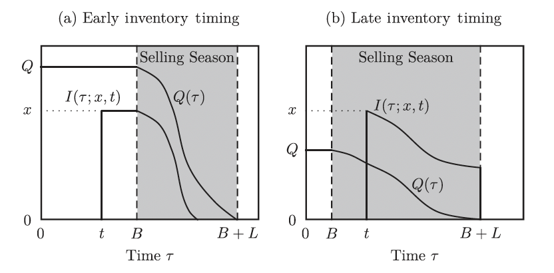
\includegraphics[width=7.5cm]{imgs/gp01-1.png}
                \end{figure}
            \end{column}
            \begin{column}{0.35\linewidth}
                $I(\tau; x, t) = \left[x - (Q(t) - Q(\tau))\right]^+$ denotes the firm's inventory position at time $\tau\in [t, B+L]$ for a given inventory policy $(x, t)$
            \end{column}
        \end{columns}

    \end{frame}

    \section{\textsc{Solution}}

    \begin{frame}
        \frametitle{\textsc{Solving the stochastic season - 1}}

        \textrm{\bfseries Proposition 1} For a given $t\geq 0$, let $m(t)$  be the expected profit margin of the first sold item; that is, $m(t) = p - c - h\int_{t}^{b_u} \mathbb P(B > b)\dd b$ if $t\in [0, b_u]$, $m(t) = p - c$ if $t\in (b_u, b_u + l_u)$, and $m(t) = 0$ otherwise. For a fixed inventory timing $t$, the optimal inventory quantity $x^*(t)$ is determined uniquely as a function of $t$ which satisfies

        \begin{enumerate}
            \item for any $t$ such that $m(t) \leq 0, x^*(t) = 0$
            \pause
            \item for any $t$ such that $m(t) > 0, x^*(t)$ solves \eqnref{eq:1}
        \end{enumerate}

        \begin{equation}
            \begin{aligned}
                & \mathbb P(Q(t)\leq x^*(t)) \\
                =& \frac{p - c - h\left[\int_{t}^{b_u}\mathbb P(B>b)\dd b + \mathbb E_{B, L}\left[\int_{\max\{t, B\}}^{B+L} \mathbb P(Q(t) - Q(\tau) \leq x^*(t) | B, L)\dd \tau\right]\right]}{p-s}
            \end{aligned}
            \label{eq:1}
        \end{equation}

    \end{frame}

    \begin{frame}
        \frametitle{\textsc{Solving the stochastic season - 1}}

        \eqnref{eq:1} can be written as \eqnref{eq:2}

        \begin{equation}
            \mathbb P(Q(t)\leq x^*(t)) = \frac{m(t)}{p-s} - \frac{h}{p-s}\mathbb E_{B, L}\times \left[\int_{\max\{t, B\}}^{B+L} \mathbb P(Q(t) - Q(\tau)\leq x^*(t) | B, L)\dd \tau\right]
            \label{eq:2}
        \end{equation}

        \pause

        $\mathbb P(Q(t)\leq x^*(t))$ satisfies

        \begin{enumerate}
            \item $(m(t) - hl_u)^+ / (p-s)\leq \mathbb P(Q(t)\leq x^*(t))\leq m(t) / (p-s)$
            \item Specifically, when $h = 0$, $\mathbb P(Q(t)\leq x^*(t)) = m(t) / (p-s) = (p-c)/(p-s)$
        \end{enumerate}

    \end{frame}

    \begin{frame}
        \frametitle{\textsc{Solving the stochastic season - 2}}

        \textrm{\bfseries Proposition 2} The optimal inventory timing $t^*$ satisfies optimality condition \eqnref{eq:3}:

        \begin{equation}
            \begin{aligned}
                & hx^*\left(t^*\right)\mathbb P(t^*\leq B+L) - h\mathbb E_{B, L}\int_{t^*}^{B+L} \left[\begin{aligned}
                    & \mathbb E_Q \left[D\left(t^*\right)\middle | Q\left(t^*\right) - Q(\tau)\leq x^*\left(t^*\right), B\leq t^*, L\right] \\
                    & \times \mathbb P\left(Q\left(t^*\right) - Q(\tau)\leq x^*\left(t^*\right), B\leq t^*\right)
                \end{aligned}\right] \dd \tau \\
                =& (p-s)\mathbb E_{Q, B, L}\left[D\left(t^*\right)\middle | Q\left(t^*\right)\leq x\right]\mathbb P\left(Q\left(t^*\right)\right)\leq x^*\left(t^*\right)
            \end{aligned}
            \label{eq:3}
        \end{equation}

        $t^*$ satisfies that $t^* > 0\Leftrightarrow h > 0$

    \end{frame}

    \begin{frame}
        \frametitle{\textsc{Solving the stochastic season - 3}}

        \textrm{\bfseries Lemma 1} Let $f_Y$ be the PDF of the random variable $Y$. The firm's optimal inventory quantity $x^*(t)$ increases with $t$ if and only if \eqnref{eq:4} stands.

        \begin{equation}
            \begin{aligned}
                & h\mathbb P(t < B+L) - h\mathbb E_{B, L}\int_t^{B+L}\left[\begin{aligned}
                    & \mathbb E_Q\left[D(t)\middle|Q(t) - Q(\tau) \leq x^*(t), B\leq t, L\right] \times \\
                    & f_{Q(t)-Q(\tau)|B\leq t}\left(x^*(t)\right)\mathbb P(B\leq t)
                \end{aligned}\right]\dd \tau \\
                &> (p-s)\mathbb{E}_{Q, B, L}\left[D(t)\middle| Q(t)\leq x^*(t)\right]f_{Q(t)}\left(x^*(t)\right)
            \end{aligned}
            \label{eq:4}
        \end{equation}

        \pause

        In particular:

        \begin{enumerate}
            \item $h = 0\Rightarrow \dd x^*(t) / \dd t \leq 0$
            \item $h > 0\Rightarrow \exists \underline{t} > 0, \forall t\in [0, \underline t], x^{*\prime}(t) \geq 0$
        \end{enumerate}
    \end{frame}

    \begin{frame}
        \frametitle{\textsc{Solving the stochastic season - 4}}

        \textrm{\bfseries Proposition 3} For a given inventory policy $(x, t)$, the firm's expected lost sales are given by $\mathcal L(x, t) = \mathbb E_{Q, B, L}\left[(Q - Q(t)) + \left[Q(t) - x\right]^+\right]$. $\mathcal L\left(x^*(t), t\right)$ decreases with $t$ if and only if \eqnref{eq:5} stands.

        \begin{equation}
            \frac{\dd x^*(t)}{\dd t} > \frac{\mathbb E_{Q, B, L}\left[D(t)\middle| Q(t)\leq x^*(t)\right]\mathbb P\left(Q(t)\leq x^*(t)\right)}{\mathbb P\left(Q(t) > x^*(t)\right)}
            \label{eq:5}
        \end{equation}

        \pause

        In particular:

        \begin{enumerate}
            \item $h = 0\Rightarrow \mathcal L\left(x^*(t), t\right)$ increases with $t$
            \item $h > 0\Rightarrow \exists t_1 > 0, \forall t\in [0, t_1], L\left(x^*(t), t\right)$ decreases with $t$.
        \end{enumerate}

    \end{frame}

    \subsection{\textsc{Simplification}}

    \begin{frame}
        \frametitle{\textsc{Impact of customer demand pattern}}

        The conditions that characterize the optimal inventory quantity and timing for a firm that faces a stochastic selling season are rather complex

        There are two special cases that are both instructive and practically relevant

        \begin{enumerate}
            \item Instantaneous demand which is similar to newsvendor model except unknown beginning time $B$ of the demand
            \item Deterministic selling season in which $A, Q, B, L$ are all given
        \end{enumerate}

    \end{frame}

    \subsubsection{\textsc{Instantaneous Demand}}

    \begin{frame}
        \frametitle{\textsc{Instantaneous demand - problem setting}}

        When demand is instantaneous, we have $L = 0$ and $A(\tau; B) = 1_{\{\tau\leq B\}}$. and optimization problem reduces to \eqnref{eq:6}

        \begin{equation}
            \max_{(x, t)\geq 0}\Pi_{i}(x, t) = \mathbb E_{Q, B}\left[(p-c)x - hx\left[B-t\right]^+ - (p-s)\left[x - Q(t)\right]^+\right]
            \label{eq:6}
        \end{equation}

        From \eqnref{eq:6}, we have

        \begin{itemize}
            \item when $h = 0$ or $h$ is low, it would set $t_i = 0$
            \item when $h$ is sufficiently high, it would set $t_i > 0$
        \end{itemize}

    \end{frame}

    \begin{frame}
        \frametitle{\textsc{Instantaneous demand - optimal solution}}

        Assume that $h - (p-s)f_B(0) > 0$, let $H_Y = f_Y / (1 - F_Y)$ denote the hazard rate of the random variable $Y$, in which $F_Y$ being the CDF of the random variable $Y$. The firm's optimal inventory policy solves

        \begin{align}
            \mathbb P\left(Q\left(t_i\right)\leq x_i\right) &= \frac{p - c - h\int_{t_i}^{b_u} \mathbb P(B>b)\dd b}{p - s} \\
            H_B\left(t_i\right) &= \frac{hx_i}{(p-s)\int_{0}^{x_i}\mathbb P(Q > q|B > t_i)\dd q}
        \end{align}

        Furthermore, $H_B'\left(t_i\right)\geq 0$

    \end{frame}

    \subsubsection{\textsc{Deterministic Selling Season}}

    \begin{frame}
        \frametitle{\textsc{Deterministic selling season - problem setting}}

        When the selling season is deterministic, we have $Q = q > 0, B = 0, L = l > 0$. The optimization problem reduces to \eqnref{eq:7}

        \begin{equation}
            \max_{(x, t)\geq 0}\Pi_d(x, t) = (p-c)x - h\int_t^l I(\tau; x, t)\dd \tau - (p - s)\left[x - A(t)q\right]^+
            \label{eq:7}
        \end{equation}

    \end{frame}

    \begin{frame}
        \frametitle{\textsc{Deterministic selling season - optimal solution}}

        Assume that $p - c \geq hl$, the firm's optimal inventory policy solves

        \begin{align}
            x_d &= A\left(t_d\right)q \\
            -\frac{A'\left(t_d\right)}{A\left(t_d\right)} &= \frac{h}{p-c}
        \end{align}

        Moreover:

        \begin{enumerate}
            \item $h = 0\Leftrightarrow t_d = 0$
            \item $A(\tau)$ is log-concave at $\tau = t_d$
            \item $t_d$ increases with $h$, $x_d$ decreases with $h$
        \end{enumerate}

    \end{frame}

    \section{\textsc{Simulation and Benchmark}}

    \begin{frame}
        \frametitle{\textsc{Simulation settings}}

        \begin{itemize}
            \item Sales price $p=\$100$, salvage cost $s = \$0$, production cost $c\in \{\$25, \$50, \$75\}$, holding cost $h = \rho c, \rho\in \{1\%, 2\%, 3\%\}$
            \item Selling season length $L\in \{0.8, 1.5, 3\}$, beginning time $B\sim B1(b_u, \alpha, \beta), b_u\in \{1, 1.5, 2\}, (\alpha, \beta)\in \{(1, 1), (2, 4), (4, 2)\}$
            \item $Q\sim \Gamma(\alpha, \beta)$, $\alpha/\beta = 100, \sqrt{\alpha / \beta^2} \in \{10, 30, 50\}$
            \item Three demand patterns:
            \begin{itemize}
                \item Constant: $D(\tau) = Q/L$
                \item Increasing: $D(\tau) = 2Q(\tau - B)/L^2$
                \item Decreasing: $D(\tau) = 2Q(B + L - \tau)/L^2$
            \end{itemize}
        \end{itemize}

        Benchmark policies: nv-policy ($h = 0$), and h-nv policy ($h > 0, t_h = 0$)

    \end{frame}

    \begin{frame}
        \frametitle{\textsc{Simulation result}}

        \begin{figure}[ht]
            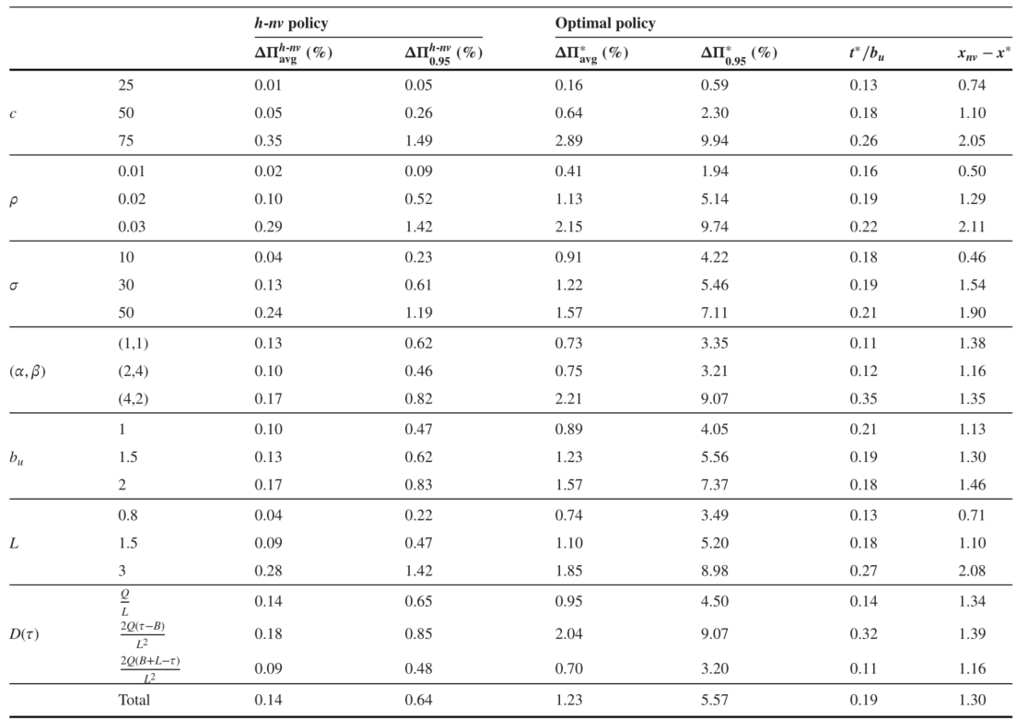
\includegraphics[width=0.65\linewidth]{imgs/gp01-2.png}
        \end{figure}

    \end{frame}

    \begin{frame}
        \frametitle{\textsc{Simulation result}}

        \begin{columns}
            \begin{column}{0.45\linewidth}
                \begin{figure}[ht]
                    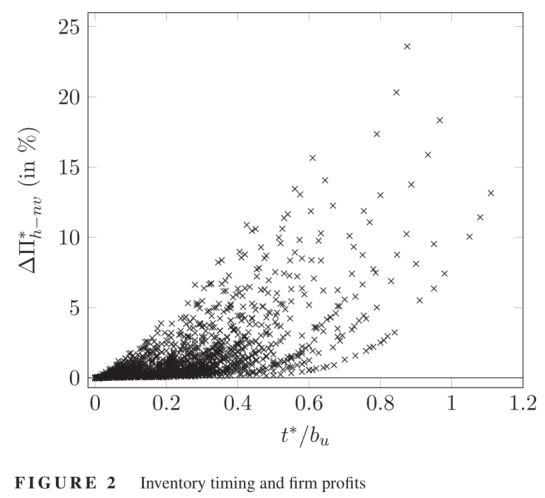
\includegraphics[width=\linewidth]{imgs/gp01-3.png}
                \end{figure}
            \end{column}
            \begin{column}{0.45\linewidth}
                \begin{figure}[ht]
                    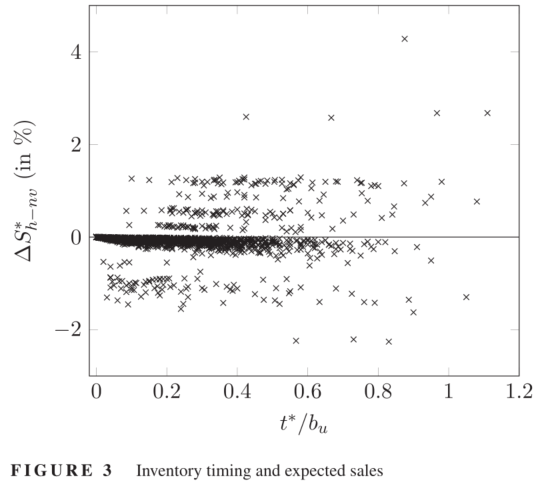
\includegraphics[width=\linewidth]{imgs/gp01-4.png}
                \end{figure}
            \end{column}
        \end{columns}

    \end{frame}

    \section{\textsc{Implications}}

    \begin{frame}
        \frametitle{\textsc{Implications}}

        \begin{enumerate}
            \item The goals of this paper are to establish the importance of a firm's inventory timing decision and to show that inventory timing has a first-order effect on both firm profits and customer service
            \item Establishing the firm's optimal inventory policy, unravel the interaction effects between the firm's inventory quantity and inventory timing
            \item Demonstrate that an optimally chosen inventory timing enables the firm to increase profits and simultaneously reduce lost sales, and disentangle how the various properties of a selling season affect a firm's inventory policy
        \end{enumerate}

    \end{frame}

    \section{\textsc{Reference}}

    \begin{frame}[allowframebreaks]
        \frametitle{\textsc{Reference}}
        {
            \setstretch{1}
            \scriptsize
            \bibliography{GP01.bib}
            \bibliographystyle{plain}
        }
    \end{frame}

    \section{\textsc{Appendix}}

    \begin{frame}
        \frametitle{\textsc{Proof of proposition 1}}

        The firm's expected profit can be rewritten as \eqnref{eq:8}

        \begin{equation}
            \begin{aligned}
                \Pi(x, t) &= \mathbb E_{Q, B, L}\left[(p-c)x - h\int_{\max\{t, B\}}^{B+L} I(\tau; x, t)\dd \tau -(p-s)\left[x-Q(t)\right]^+ - hx\left[B-t\right]^+\right] \\
            \end{aligned}
            \label{eq:8}
        \end{equation}

    \end{frame}

    \begin{frame}
        \frametitle{\textsc{Proof of proposition 1}}

        \begin{equation}
            \begin{aligned}
                \frac{\partial\Pi(x, t)}{\partial x} &= \mathbb E_{Q, B, L}\left[(p-c) - h\int_{\max\{t, B\}}^{B+L} 1_{\{Q(t) - Q(\tau)\leq x\}}\dd \tau -(p-s)1_{\{Q(t)\leq x\}} - hx\left[B-t\right]^+\right] \\
                &\begin{aligned}
                    =&(p-c) - h\mathbb E_{B, L}\times\left[\int_{\max\{t, B\}}^{B+L}\mathbb P(Q(t) - Q(\tau) \leq x|B, L)\dd \tau\right] - \\
                    &(p-s)\mathbb P(Q(t)\leq x) - h\int_t^{b_u}\mathbb P(B > b)\dd b
                \end{aligned}
            \end{aligned}
        \end{equation}

        Taking derivative yields

        \begin{equation}
            \frac{\partial^2\Pi(x, t)}{\partial x^2} = -(p-s)f_{Q(t)}(x) - h\mathbb E_{B, L}\times \left[\int_{\max\{t, B\}}^{B+L}f_{Q(t) - Q(\tau) | B, L}(x)\dd \tau\right]
        \end{equation}

    \end{frame}

    \begin{frame}
        \frametitle{\textsc{Proof of proposition 2}}

        By optimality and the envelop theorem, we have

        \begin{equation}
            \left\{
            \begin{aligned}
                \frac{\partial \Pi(x^*(t^*), t^*)}{\partial x} &= 0 \\
                \frac{\dd\Pi(x^*(t^*), t^*)}{\dd x} &= \frac{\partial \Pi(x^*(t^*), t^*)}{\partial t} = 0 \\
            \end{aligned}
            \right.
        \end{equation}

        $\mathbb E_{Q, B, L}\left[\int_{\max\{t, B\}}^{B+L} I(\tau; x, t)\dd \tau\right]$ can be rewritten as:

        \begin{equation}
            \begin{aligned}
            \mathbb E_{Q, B, L}\left[\int_{\max\{t, B\}}^{B+L} I(\tau; x, t)\dd \tau\right] =& \mathbb E_{Q, B, L}\left[\int_B^{B+L} I(\tau; x, t)\dd \tau\middle| B > t\right]\mathbb P(B > t) + \\
            & \mathbb E_{Q, B, L}\left[\int_t^{B+L} I(\tau; x, t)\dd \tau\middle| B \leq t\right]\mathbb P(B \leq t)
            \end{aligned}
        \end{equation}

    \end{frame}

    \begin{frame}
        \frametitle{\textsc{Proof of proposition 2}}

        First-order partial derivative of $\Pi(x, t)$ with respect to $t$ can be written as

        \begin{equation}
            \begin{aligned}
                \frac{\partial \Pi(x, t)}{\partial t} =& -(p-s)\mathbb E_{Q, B, L}\left[D(t) | Q(t)\leq x\right]\mathbb P(Q(t)\leq x) \\
                &+ hx\mathbb P(t < B + L) - h\mathbb E_{B, L} \\
                &\times \left[\int_t^{B+L} \mathbb E_Q\left[D(t) | Q(t) - Q(\tau)\leq x, B\leq t, L\right]\right. \\
                &\times\left.\vphantom{\int_t^{B+L}}\mathbb P(Q(t) - Q(\tau)\leq x, B\leq t)\dd \tau\right]
            \end{aligned}
        \end{equation}

    \end{frame}

    \begin{frame}
        \frametitle{\textsc{Proof of lemma 1}}

        \begin{equation}
            \begin{aligned}
                \frac{\partial ^2\Pi(x, t)}{\partial x\partial t} =
                & -(p-s)\mathbb E_{Q, B, L}\left[D(t)|Q(t)\leq x\right]f_{Q(t)}(x) \\
                & + h\mathbb P(t < B + L) - h\mathbb E_{B, L} \\
                & \times \left[\int_{t}^\mathbb{B+L}\mathbb E_Q\left[D(t)|Q(t) - Q(\tau)\leq x, B\leq t, L\right]\right. \\
                & \times \left.\vphantom{\int_t^{B+L}} f_{Q(t) - Q(\tau) | B\leq t}(x)\mathbb P(B\leq t)\dd \tau\right]
            \end{aligned}
        \end{equation}

    \end{frame}

    \begin{frame}
        \frametitle{\textsc{Proof of proposition 3}}

        \begin{equation}
            \begin{aligned}
                &\frac{\dd \mathcal L(x^*(t), t)}{\dd t} \\
                =& \mathbb E_{Q, B, L}\left[D'(t)\right] + \mathbb{E}_{Q, B, L}\left[(D(t) - (x^*(t))')1_{\{Q(t) > x^*(t)\}}\right] \\
                =& \mathbb E_{Q, B, L}\left[D(t)1_{\{Q(t)\leq x^*(t)\}}\right] - (x^*(t))'\mathbb E_{Q, B, L}\left[1_{\{Q(t)>x^*(t)\}}\right] \\
                =& \mathbb E_{Q, B, L}\left[D(t) | Q(t)\leq x^*(t)\right]\mathbb P(Q(t)\leq x^*(t)) - (x^*(t))'\mathbb P(Q(t) > x^*(t))
            \end{aligned}
        \end{equation}

    \end{frame}

    \begin{frame}
        \frametitle{\textsc{Proof of proposition 4}}

        \begin{columns}
            \begin{column}{0.5\linewidth}
                \begin{figure}[h]
                    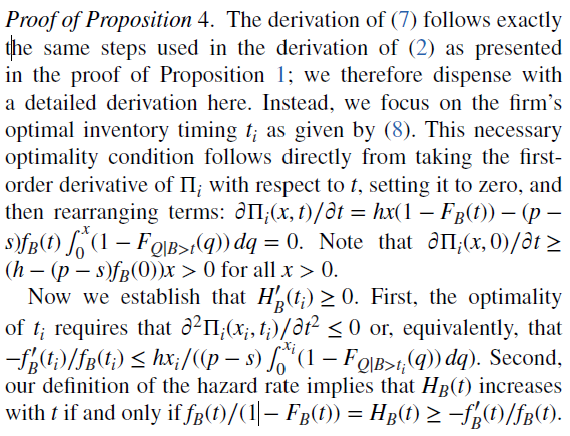
\includegraphics[width=\linewidth]{imgs/gp01-5.png}
                \end{figure}
            \end{column}
            \begin{column}{0.5\linewidth}
                \begin{figure}[h]
                    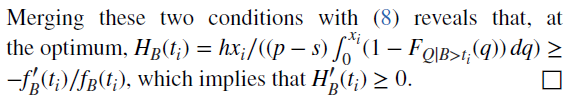
\includegraphics[width=\linewidth]{imgs/gp01-6.png}
                \end{figure}
            \end{column}
        \end{columns}

    \end{frame}

    \begin{frame}
        \frametitle{\textsc{Proof of proposition 5}}

        \begin{columns}
            \begin{column}{0.5\linewidth}
                \begin{figure}[h]
                    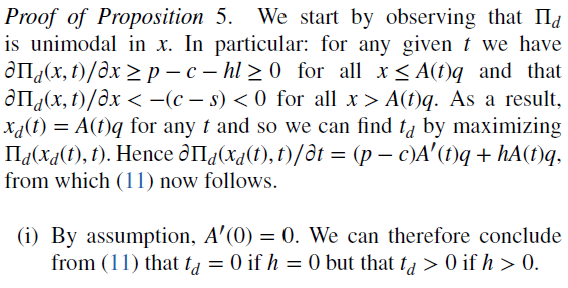
\includegraphics[width=\linewidth]{imgs/gp01-7.png}
                \end{figure}
            \end{column}
            \begin{column}{0.5\linewidth}
                \begin{figure}[h]
                    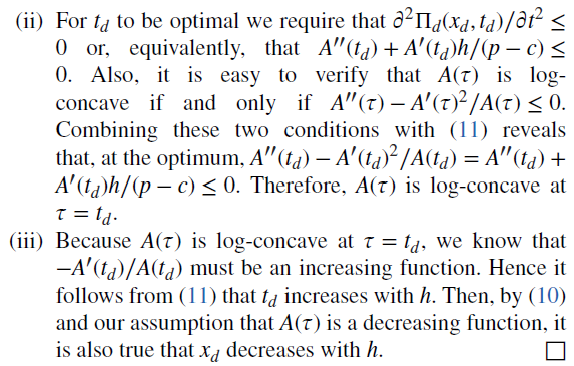
\includegraphics[width=\linewidth]{imgs/gp01-8.png}
                \end{figure}
            \end{column}
        \end{columns}

    \end{frame}
\end{document}